%----------------------------------------------------------------------------
\chapter{\bevezetes}\label{ch:bevezetes}
%----------------------------------------------------------------------------


\section{A WebRTC protokoll}\label{sec:a-webrtc-protokoll}

Napjainkban a SaaS (Software-as-a-Service) típusú szolgáltatásokra nagy mértékben jellemző a centralizáltság, elosztott
rendszerek esetében is: a felhasználók az esetek többségében egy menedzselt környezetben futó, globálisan
elérhető szerveren (legyen ez egy load balancer vagy egy egyszerű ingress-jellegű reverse proxy) keresztül lépnek
interakcióba a rendszerrel.
A centralizált jelleg a minőségbiztosítás megkönnyítése mellett hordoz egy elhanyagolhatatlan negatívumot is: ha az előbb
említett globálisan elérhető szerver meghibásodik, akkor a végfelhasználók nem tudják elérni a rendszert, hiába működik
ez hibátlanul.

Az IPv6 bevezetése és folyamatos elterjedése ugyanakkor lehetőséget biztosít arra, hogy másképp tekintsünk az internetre:
egy olyan kommunikációs hálózat, ahol akár a végfelhasználók számítógépei is képesek közvetlenül egymással kommunikálni,
NAT szüksége nélkül.

A WebRTC (RFC 7478\cite{RFC_7478}) egy olyan kommunikációs protokoll, amely lehetővé teszi két vagy több résztvevő közötti hang- és
videóhívások, illetve általános célú adatcsere megvalósítását egy köztes fél jelenléte nélkül.
Mivel a videóhívások meglehetősen széles sávszélességet igényelhetnek, a protokoll csökkenti annak az esélyét,
hogy egy köztes fél szűk keresztmetszetté váljon ennek végessége miatt.

Az előző félév Önálló Laboratóriumának keretein belül is a WebRTC protokollal foglalkoztam, ahol az elosztott nyomkövetés
problémájára kerestem egy alternatív megoldást.
Ebben a dolgozatban a protokoll használata során implementálandó signaling folyamatra keresek egy decentralizált, köztes
fél nélkül működő megoldást.

A protokoll használata során az egyes felek lehetőség szerint közvetlenül egymással kommunikálnak, peer-to-peer módon.
A kommunikációs csatorna az ICE (RFC 8445\cite{ICE}) protokoll használatával van felépítve, amely során a felek egy STUN (RFC 5389)
szerver segítségével felderítik a saját publikus IP címüket és olyan port-ot, amelyen globálisan elérhetőek.
Amennyiben valamely fél olyan NAT környezetben van, amelyben nem valósítható meg a peer-to-peer kommunikáció, mint például
a szimmetrikus NAT típusok, a két fél egy köztes TURN (RFC 5766\cite{TURN}) szerveren keresztül kommunikál egymással, amely egy
relay-jellegű funkcionalitást valósít meg.
Az~\ref{fig:ice}-es ábra az ICE protokoll működését mutatja be.

\begin{figure}[!ht]
    \centering
    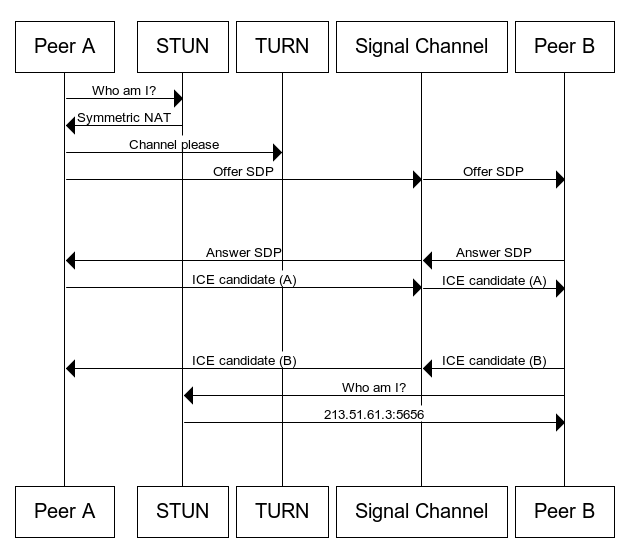
\includegraphics[width=150mm, keepaspectratio]{figures/ice}
    \caption{Az ICE folyamat ábrázolva (forrás: \href{https://developer.mozilla.org/en-US/docs/Web/API/WebRTC_API/Connectivity}{developer.mozilla.org})}
    \label{fig:ice}
\end{figure}

A kommunikáció felépítésének (más néven \emph{signaling}) során szükség van egy out-of-band, \textbf{kétirányú}
kommunikációs csatornára, amelyen keresztül a résztvevők elküldik egymásnak az ICE folyamat során szerzett ICE candidate-eket.
Ezt a csatornát a WebRTC protokoll \emph{nem biztosítja}.
A gyakorlatban ez a csatorna általában a WebSocket protokoll (RFC 6455\cite{WebSocket}) használatával, vagy HTTP long-polling-gal van
implementálva.

Ideális NAT körülmények között a signaling-ot megvalósító szerver az egyetlen centralizált komponens egy WebRTC protokollt
alkalmazó rendszerben, mivel egy köztes relay-re soha nem lesz szükség, a STUN szerver terhelése és sávszélesség-igénye
pedig elenyésző valósidejű hang- és képátvitel esetén.

Ha két fél képes megvalósítani a signaling-ot egy köztes, dedikált szolgáltatás nélkül, akkor ez \emph{a két fél képes közvetlenül
kommunikálni egymással, függetlenül attól, hogy földrajzilag hol helyezkedik el, az IP címek konfigurációja nélkül
\footnote{Feltételezve, hogy stabil internetkapcsolattal, áramellátással és ideális (vagy nem létező) NAT körülményekkel rendelkeznek.}}.

Jelen dolgozat a dedikált signaling szerver elosztott hash-táblákkal (továbbiakban DHT) történő helyettesítésének egy
lehetséges eljárását mutatja be.
